\documentclass[10pt,pdf,hyperref={unicode}]{beamer}

\mode<presentation>
{
\usetheme{boxes}
\beamertemplatenavigationsymbolsempty

\setbeamertemplate{footline}[page number]
% \usecolortheme{seagull}
\setbeamersize{text margin left=0.5em, text margin right=0.5em}
}

\usepackage[utf8]{inputenc}
\usepackage[english, russian]{babel}
\usepackage{bm}
\usepackage{multirow}
\usepackage{ragged2e}
\usepackage{indentfirst}
\usepackage{multicol}
\usepackage{subfig}
\usepackage{amsmath}

\usepackage{tikz}
\usetikzlibrary{positioning,arrows}

\tikzstyle{name} = [parameters]
\definecolor{name}{rgb}{0.5,0.5,0.5}

\newtheorem{rustheorem}{Теорема}
\newtheorem{rusdefinition}{Определение}

\AtBeginEnvironment{figure}{\setcounter{subfigure}{0}}% Resets subfigure counter at start of figure environment

\captionsetup[subfloat]{labelformat=empty}

%----------------------------------------------------------------------------------------------------------

\title[Априорное распределение параметров модели]{Байесовский выбор\\ априорного распределения параметров}
\author{А.\,В.\,Грабовой}

\institute[]{Диссертация на соискание ученой степени\\
кандидата физико-математических наук\\05.13.17 --- Теоретические основы информатики\\Научный руководитель: д.ф.-м.н. В.В. Стрижов\\}     
%\institute[МФТИ]{Московский Физико-Технический Институт (Государственный Университет)}
\date[2021]{Московский физико-технический институт\\21 сентября 2021 г.}

%----------------------------------------------------------------------------------------------------------

\begin{document}
%----------------------------------------------------------------------------------------------------------
\begin{frame}
\titlepage
\end{frame}

%----------------------------------------------------------------------------------------------------------
\begin{frame}{Выбор априорного распределения параметров v1}
\justifying

\textbf{Исследуемая проблема}

\textbf{Цель:} предложить метод выбора начального приближения моделей глубокого обучения.\\
\textbf{Задачи}
\begin{enumerate}
\item Предложить байесовский метод обучения моделей ученика на основе моделей учителя.
\item Предложить алгоритм построения модели на основе предобученных моделей.
\end{enumerate}
\textbf{Исследуемые проблемы}
\begin{enumerate}
\item Большое число параметров и гиперпараметров модели, высокая вычислительная сложность оптимизации.
\item Многоэкстремальность и невыпуклость задачи оптимизации.
\end{enumerate}
\textbf{Методы исследования}\\ 
Используются методы байесовского вывода. Для получения начального приближения модели глубокого обучения используется априорное распределение параметров, которое получается как апостериорное распределения ранее обученной модели.
\end{frame}

%----------------------------------------------------------------------------------------------------------
\begin{frame}{Выбор априорного распределения параметров v2}
\justifying

\textbf{Исследуемая проблема}

\textbf{Цель:} предложить метод выбора априорного распределения параметров моделей глубокого обучения.\\
\textbf{Задачи}
\begin{enumerate}
\item Предложить метод сопоставления параметрических моделей на основе байесовского вывода.
\item Предложить метод снижения размерности пространства параметров нейросетевых моделей.
\end{enumerate}
\textbf{Исследуемые проблемы}
\begin{enumerate}
\item Большое число параметров и гиперпараметров модели, высокая вычислительная сложность оптимизации.
\item Многоэкстремальность и невыпуклость задачи оптимизации.
\end{enumerate}
\textbf{Методы исследования}\\ 
Используются методы байесовского вывода. Для получения начального приближения модели глубокого обучения используется априорное распределение параметров, которое получается на основе апостериорного распределения предобученной. 
\end{frame}

%----------------------------------------------------------------------------------------------------------
\begin{frame}{Выбор априорного распределения параметров v3}
\justifying

\textbf{Исследуемая проблема}

\textbf{Цель:} предложить метод автоматического назначения априорного распределения параметров в моделях глубокого обучения.\\
\textbf{Задачи}
\begin{enumerate}
\item Предложить метод сопоставления параметрических моделей на основе байесовского вывода.
\item Предложить метод выбора априорного распределения параметров модели используя экспертную информацию о задаче.
\end{enumerate}
\textbf{Исследуемые проблемы}
\begin{enumerate}
\item Большое число параметров и гиперпараметров модели, высокая вычислительная сложность оптимизации.
\item Многоэкстремальность и невыпуклость задачи оптимизации.
\end{enumerate}
\textbf{Методы исследования}\\ 
Используется байесовский подход к обучению нейросетевых моделей. Априорное распределение параметров модели назначается на основе экспертной информации о рассматриваемой задаче. В частности в качестве экспертной информации рассматриваются предобученные параметрические модели.
\end{frame}

%----------------------------------------------------------------------------------------------------------

\begin{frame}{Базовая постановка задачи машинного обучения}
\justifying

\begin{figure}[h!]
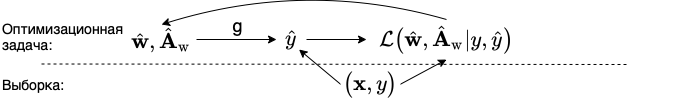
\includegraphics[width=1.0\textwidth]{figures/introdigram_low}
\end{figure}

Задана выборка:
$
	\mathfrak{D} = \left\{\textbf{x}_i, y_i\right\}_{i=1}^{m}, \quad 
	\textbf{x}_{i} \in \mathbb{R}^{n}, \quad y_i \in \mathbb{Y},
$
где~$m$~число объектов, $n$~число признаков.\\[1mm]
Модель:
$
    \mathfrak{G} = \left\{g | g : \mathbb{R}^{n}\times \mathbb{R}^{n_{w}} \to \mathbb{Y} \right\}.
$\\[1mm]
Прогноз:
$
    \hat{y} = g\bigr(\textbf{x}, \hat{\textbf{w}}).
$\\[1mm]
Функция потерь:
$
    \mathcal{L}\bigr(\hat{\textbf{w}},\hat{\textbf{A}}_{\text{w}}|y, \hat{y}\bigr).
$\\[1mm]
Оптимизационная задача:
\[
    \hat{\textbf{w}}, \hat{\textbf{A}}_{w} = \arg \min_{\textbf{w} \in \mathbb{R}^{n_{w}}, \textbf{A} \in \mathbb{R}^{n_{w}\times n_{w}}} \mathcal{L}\bigr(\textbf{w},\textbf{A}_{\text{w}}|y, \hat{y}\bigr).
\]
\end{frame}

%----------------------------------------------------------------------------------------------------------


\begin{frame}{Априорное распределение параметров}
\justifying

\begin{figure}[h!]
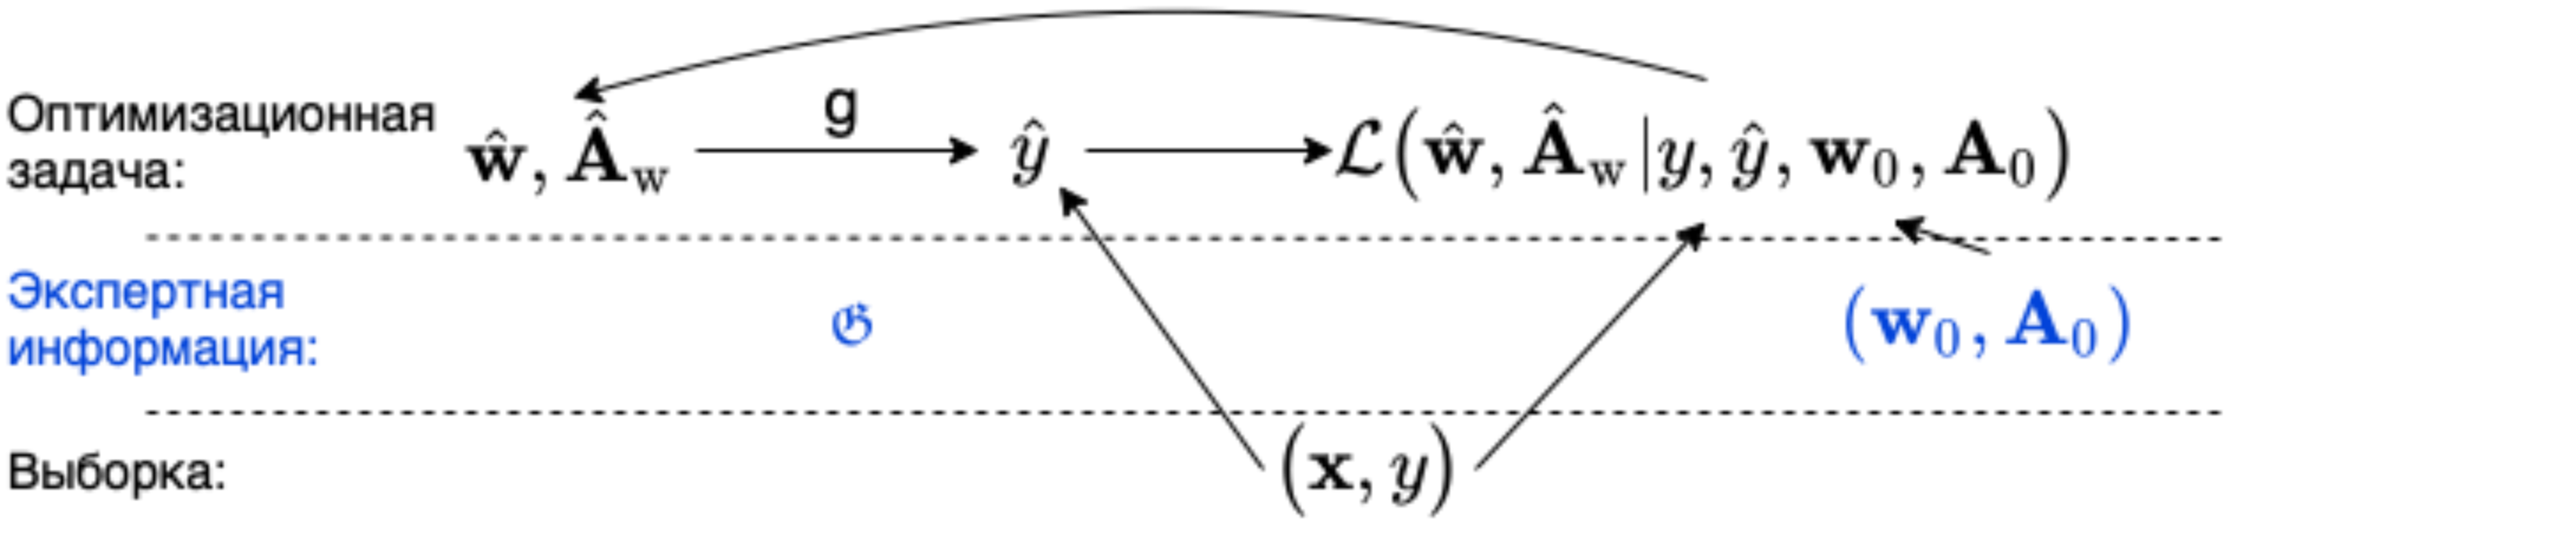
\includegraphics[width=1.0\textwidth]{figures/introdigram}
\end{figure}

Задана выборка:
$
	\mathfrak{D} = \left\{\textbf{x}_i, y_i\right\}_{i=1}^{m}, \quad 
	\textbf{x}_{i} \in \mathbb{R}^{n}, \quad y_i \in \mathbb{Y},
$
где~$m$~число объектов, $n$~число признаков.\\[1mm]
Модель:
$
    \mathfrak{G} = \left\{g | g : \mathbb{R}^{n}\times \mathbb{R}^{n_{w}} \to \mathbb{Y} \right\}.
$\\[1mm]
{\color{blue}
Априорное распределение параметров модели:
$
    \textbf{w} \sim \mathcal{N}\bigr(\textbf{w}_0, \textbf{A}_0\bigr).
$\\[1mm]
}
Прогноз:
$
    \hat{y} = g\bigr(\textbf{x}, \hat{\textbf{w}}).
$\\[1mm]
Функция потерь:
$
    \mathcal{L}\bigr(\hat{\textbf{w}},\hat{\textbf{A}}_{\text{w}}|y, \hat{y}, {\color{blue}\textbf{w}_0, \textbf{A}_0}\bigr).
$\\[1mm]
Оптимизационная задача:
\[
    \hat{\textbf{w}}, \hat{\textbf{A}}_{w} = \arg \min_{\textbf{w} \in \mathbb{R}^{n_{w}}, \textbf{A} \in \mathbb{R}^{n_{w}\times n_{w}}} \mathcal{L}\bigr(\hat{\textbf{w}},\hat{\textbf{A}}_{\text{w}}|y, \hat{y}, {\color{blue}\textbf{w}_0, \textbf{A}_0}\bigr).
\]
\end{frame}

%----------------------------------------------------------------------------------------------------------

\begin{frame}{Байесовская дистилляция модели}
\justifying
\begin{figure}[h!]

\includegraphics[width=1.0\textwidth]{slides/figures/introdigram_large}
\end{figure}

Задана выборка:
$
	\mathfrak{D} = \left\{\textbf{x}_i, {\color{blue}\textbf{x}_i^{*}}, y_i\right\}_{i=1}^{m}, 
	\quad \textbf{x}_{i} \in \mathbb{R}^{n}, 
	{\color{blue}\quad \textbf{x}_{i}^{*} \in \mathbb{R}^{n^{*}}},
	\quad y_i \in \mathbb{Y}.
$\\[1mm]
Модели ученика и учителя:
$
    \mathfrak{G} = \left\{g | g : \mathbb{R}^{n}\times \mathbb{R}^{n_{w}} \to \mathbb{Y} \right\},
{\color{blue}
    \quad \mathfrak{F} = \left\{f | f : \mathbb{R}^{n^{*}}\times \mathbb{R}^{n_{w}^{*}} \to \mathbb{Y} \right\}.
}
$\\[1mm]
{\color{blue}
Задана оптимальная функция учителя~$f \in \mathfrak{F}.$
}
\\[1mm]
Априорное распределение параметров модели:
$
    \textbf{w} \sim \mathcal{N}\bigr({\color{blue}\textbf{w}_0\bigr(\hat{\textbf{u}}, \hat{\textbf{A}}_{\text{u}}\bigr)}, {\color{blue}\textbf{A}_0\bigr(\hat{\textbf{u}}, \hat{\textbf{A}}_{\text{u}}\bigr)}\bigr).
$\\[1mm]
Прогноз:
$
    \hat{y} = g\bigr(\textbf{x}, \hat{\textbf{w}}).
{\color{blue}
    \quad
    s = f\bigr(\textbf{x}^{*}, \hat{\textbf{u}}).
}
$\\[1mm]
Функция потерь:
$
    \mathcal{L}\bigr(\hat{\textbf{w}},\hat{\textbf{A}}_{\text{w}}|{\color{blue} s, }y, \hat{y}, {\color{blue}\textbf{w}_0, \textbf{A}_0}\bigr).
$[1mm]
Оптимизационная задача:
\[
    \hat{\textbf{w}}, \hat{\textbf{A}}_{w} = \arg \min_{\textbf{w} \in \mathbb{R}^{n_{w}}, \textbf{A} \in \mathbb{R}^{n_{w}\times n_{w}}} \mathcal{L}\bigr(\hat{\textbf{w}},\hat{\textbf{A}}_{\text{w}}|{\color{blue} s, }y, \hat{y}, {\color{blue}\textbf{w}_0, \textbf{A}_0}\bigr).
\]
\end{frame}

%----------------------------------------------------------------------------------------------------------

\begin{frame}{Оптимизация ученика на основе учителя}
\justifying
Заданы:
\begin{enumerate}
    \item[1)] признаки~$\textbf{x}_i \in \mathbb{R}^{n}$;
    \item[2)] привилегированные признаки~$\textbf{x}^*_i \in \mathbb{R}^{n^*}$;
    \item[3)] целевая переменная~$y_i \in \mathbb{Y}$;
    \item[4)] индексы объектов, для которых известна привилегированная информация $\mathcal{I},$ а для которых она не известна $\bar{\mathcal{I}}$.
\end{enumerate}

\bigskip

Функции учителя~$\textbf{f}:\mathbb{R}^{n^*} \to \mathbb{Y}^\prime$ и ученика~$\textbf{g}:\mathbb{R}^{n} \to \mathbb{Y}^\prime$ --- пространство оценок.

Ответ $\textbf{s}_i = \textbf{f}\bigr(\textbf{x}_i^*\bigr)$ функции $\textbf{f}$ для объекта~$\textbf{x}^*_i$ используется при решении оптимизационной задачи.

\bigskip

Требуется выбрать модель ученика~$\textbf{g}$ из множества
\[
	\mathfrak{G} = \left\{\textbf{g}| \textbf{g}:\mathbb{R}^{n} \to \mathbb{Y}^\prime\right\}.
\]

Оптимизационная задача:
\[
	\textbf{g} = \arg\min_{\textbf{g} \in \mathfrak{G}} \mathcal{L}\bigr(\textbf{g}, \textbf{f}, \textbf{X}, \textbf{X}^{*}, \textbf{y}\bigr),
\]
где $\mathcal{L}$ функция ошибки.
\end{frame}
%----------------------------------------------------------------------------------------------------------
\begin{frame}{Постановка задачи: дистилляция {\color{blue}Хинтона}\footnotemark; {\color{red}Вапника}\footnotemark}
\justifying
Заданы:
\begin{enumerate}
	\item[1)] {\color{blue} $\textbf{x}^*_i = \textbf{x}_i$}; {\color{red} $\textbf{x}^*_i \not= \textbf{x}_i$} для всех $i \in \{1, 2, \cdots, m\}$;
	\item[2)] $y_i \in \mathbb{Y}=\{1, \cdots, K\}, \quad \mathbb{Y}^\prime=\mathbb{R}^{K}$.
\end{enumerate}

Параметрические семейства учителя и ученика:
\[
\setlength\abovedisplayskip{0pt}
\mathfrak{F}^{\color{red}*}_{\text{cl}} = \left\{\textbf{f}| \textbf{f} = \text{softmax}\bigr(\textbf{v}^{\color{red}*}\bigr(\textbf{x}^{\color{red}*}\bigr)/T\bigr), \quad \textbf{v}^{\color{red}*}: \mathbb{R}^{n^{\color{red}*}} \to \mathbb{R}^K \right\},
\setlength\belowdisplayskip{0pt}
\]
\[
\setlength\abovedisplayskip{0pt}
\mathfrak{G}_{\text{cl}} = \left\{\textbf{g}| \textbf{g} = \text{softmax}\bigr(\textbf{z}\bigr(\textbf{x}\bigr)/T\bigr), \quad \textbf{z}: \mathbb{R}^n \to \mathbb{R}^K \right\},
\setlength\belowdisplayskip{0pt}
\]
где~$\textbf{z},\textbf{v}^{\color{red}*}$~--- это дифференцируемые параметрические функции заданной структуры, $T$~--- параметр температуры.

Функция ошибки
\[
\setlength\abovedisplayskip{0pt}
\begin{aligned}
   \mathcal{L}_\text{st}\bigr(\textbf{g}\bigr) = &-\sum_{i=1}^{m}\underbrace{{\sum_{k=1}^{K}y^k_i\log\textbf{g}\bigr(\textbf{x}_i\bigr)\bigr|_{T=1}}}_{\text{исходная функция потерь}}- \sum_{i=1}^{m}\underbrace{{\sum_{k=1}^{K}\textbf{f}\bigr(\textbf{x}^{\color{red}*}_i\bigr)\bigr|_{T=T_0}\log\textbf{g}\bigr(\textbf{x}_i\bigr)\bigr|_{T=T_0}}}_{\text{слагаемое дистилляция}},
\end{aligned}
\setlength\belowdisplayskip{0pt}
\]
где~$\cdot\bigr|_{T=t}$ параметр температуры~$T$ равняется~$t$.

Оптимизационная задача:
\[
\setlength\abovedisplayskip{0pt}
	\hat{\textbf{g}} = \arg\min_{\textbf{g} \in \mathfrak{G}_{\text{cl}}} \mathcal{L}_\text{st}\bigr(\textbf{g}\bigr).\setlength\belowdisplayskip{0pt}
\]
\footnotetext[1]{\textit{Hinton G., Vinyals O., Dean J.} Distilling the Knowledge in a Neural Network // NIPS, 2015.}
\footnotetext[2]{\textit{Lopez-Paz D., Bottou L., Scholkopf B., Vapnik V.} Unifying Distillation and Privileged Information //ICLR, 2016.}
\end{frame}
%----------------------------------------------------------------------------------------------------------
\begin{frame}{Вероятностная постановка задачи дистилляции}
\justifying
Гипотеза порождения данных:
\begin{enumerate}
	\item[1)] задано распределение целевой переменной~$p\bigr(y_i|\textbf{x}_i, \textbf{g}\bigr)$;
	\item[2)] задано совместное распределение~$p\bigr(y_i, \textbf{s}_i|\textbf{x}_i, \textbf{g}\bigr)$;
	\item[3)] для всех $i \in \mathcal{I}$ элементы $y_i$ и $\textbf{s}_i$ являются зависимыми величинами;
	\item[4)] если $|\mathcal{I}|=0$ то решение равно решению максимума правдоподобия.
\end{enumerate}
Совместное правдоподобие истинных меток и меток учителя:
\[
\setlength\abovedisplayskip{0pt}
p\bigr(\textbf{y}, \textbf{S}|\textbf{X}, \textbf{g}, \mathcal{I}\bigr)=\prod_{i\not\in \mathcal{I}}p\bigr(y_i|\textbf{x}_i, \textbf{g}\bigr)\prod_{i\in \mathcal{I}}p\bigr(y_i, \textbf{s}_i|\textbf{x}_i, \textbf{g}\bigr).
\setlength\belowdisplayskip{0pt}
\]

\begin{columns}
\column{0.55\textwidth}
Задача оптимизации:
\[
\setlength\abovedisplayskip{0pt}
\textbf{g} = \arg\max_{\textbf{g} \in \mathfrak{G}} p\bigr(\textbf{y}, \textbf{S}|\textbf{X}, \textbf{g}, \mathcal{I}\bigr),
\setlength\belowdisplayskip{0pt}
\]
имеет вид:
\[
\setlength\abovedisplayskip{0pt}
\begin{aligned}
\sum_{i\not\in \mathcal{I}}\log p\bigr(y_i|\textbf{x}_i, \textbf{g}\bigr) &+ \left(1-\lambda\right)\sum_{i\in \mathcal{I}}\log p\bigr(y_i|\textbf{x}_i, \textbf{g}\bigr) \\
&+ \lambda\sum_{i\in \mathcal{I}}\log p\bigr(\textbf{s}_i|\textbf{x}_i, \textbf{g}\bigr),
\end{aligned}
\setlength\belowdisplayskip{0pt}
\]
где~$\lambda \in [0,1]$ --- метапараметр.
\column{0.4\textwidth}
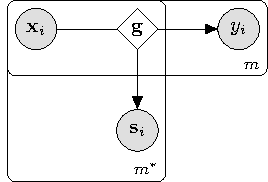
\includegraphics[width=\textwidth]{figures/proba_model}
\end{columns}

\end{frame}

%----------------------------------------------------------------------------------------------------------
\begin{frame}{Задача классификации: вероятностная постановка}
\justifying
Заданы:
\begin{enumerate}
	\item[1)] учитель $\textbf{f}\in\mathfrak{F}_{\text{cl}}^{*}$ и ученик~$\textbf{g}\in\mathfrak{G}_{\text{cl}}$;
	\item[2)] распределение истинных меток~$p\bigr(y|\textbf{x}, \textbf{g}\bigr) = \text{Cat}\bigr(\textbf{g}\bigr(\textbf{x}\bigr)\bigr)$;
	\item[3)] распределение ответов учителя~$p\bigr(\textbf{s}|\textbf{x}, \textbf{g}\bigr) = C\prod_{k=1}^{K}g_k\bigr(\textbf{x}\bigr)^{s^k}, \quad C < \infty.$
\end{enumerate}
\[
\setlength\abovedisplayskip{0pt}
\begin{aligned}
&\hat{\textbf{g}} = \arg\max_{\textbf{g}\in \mathfrak{G}} \sum_{i\not\in \mathcal{I}}\sum_{k=1}^{K}y_i^k\log g_k\bigr(\textbf{x}_i\bigr)\bigr|_{T=1} 
+ \left(1-\lambda\right)\sum_{i\in \mathcal{I}}\sum_{k=1}^{K}y_i^k\log g_k\bigr(\textbf{x}_i\bigr)\bigr|_{T=1} \\
&+ \lambda\sum_{i\in \mathcal{I}}\sum_{k=1}^{K}s_{i,k}\log g_k\bigr(\textbf{x}_i\bigr)\bigr|_{T=T_0} 
+ \lambda \sum_{i\in \mathcal{I}}\sum_{k=1}^{K}\left(\log g_k\bigr(\textbf{x}_i\bigr)\bigr|_{T=T_0} + \log\log\frac{1}{g_k\bigr(\textbf{x}_i\bigr)}\bigr|_{T=T_0}\right).
\end{aligned}
\setlength\belowdisplayskip{0pt}
\]

\begin{rustheorem}[Грабовой, 2020]
\label{theorem:st:dist}
Пусть всех $k$ выполняется $1 > 1- \varepsilon > g_k\bigr(\textbf{x}\bigr) > \varepsilon > 0,$ тогда при
\[
\setlength\abovedisplayskip{0pt}
C=\left(-1\right)^{K}\frac{K^{K/2}}{2^{K(K-1)/2}}\prod_{k=1}^{K}g_k\bigr(\textbf{x}\bigr)\log g_k\bigr(\textbf{x}\bigr)
\setlength\belowdisplayskip{0pt}
\]
функция $p\bigr(\textbf{s}|\textbf{x}, \textbf{g}\bigr) = C\prod_{k=1}^{K}g_k\bigr(\textbf{x}\bigr)^{s^k}$ является плотностью распределения.
\end{rustheorem}

\end{frame}
%----------------------------------------------------------------------------------------------------------
\begin{frame}{Задача регрессии: вероятностная постановка}
\justifying
\begin{enumerate}
	\item[1)] учитель~$f\in\mathfrak{F}_{\text{rg}}^{*}= \left\{f| f = \textbf{v}^*\bigr(\textbf{x}^*\bigr), \quad \textbf{v}^*: \mathbb{R}^{n^*} \to \mathbb{R} \right\}$;
	\item[2)] ученик~$g\in\mathfrak{G}_{\text{rg}} = \left\{g| g = \textbf{z}\bigr(\textbf{x}\bigr), \quad \textbf{z}: \mathbb{R}^n \to \mathbb{R} \right\}$;
	\item[3)] распределение истинных меток $p\bigr(y|\textbf{x}, g\bigr) = \mathcal{N}\bigr(y|g\bigr(x\bigr), \sigma\bigr)$;
	\item[4)] распределения меток учителя $p\bigr(s| \textbf{x}, g\bigr) = \mathcal{N}\bigr(s|g\bigr(\textbf{x}\bigr), \sigma_s\bigr).$
\end{enumerate}
Оптимизационная задача:
\[
\setlength\abovedisplayskip{0pt}
\begin{aligned}
\hat{g} = \arg\min_{g\in \mathfrak{G}} & \sum_{i\not\in \mathcal{I}}\sigma^2\left(y_i-g\bigr(\textbf{x}_i\bigr)\right)^2 \\
&+ \left(1-\lambda\right)\sum_{i\in \mathcal{I}}\sigma^2\left(y_i-g\bigr(\textbf{x}_i\bigr)\right)^2 + \lambda\sum_{i\in \mathcal{I}}\sigma_s^2\left(s_i-g\bigr(\textbf{x}_i\bigr)\right)^2.
\end{aligned}
\setlength\belowdisplayskip{0pt}
\]

\begin{rustheorem}[Грабовой, 2020]
\label{theorem:st:reg}
Пусть~$\mathfrak{G}_{rg}$ --- класс линейных функций~$g\bigr(\textbf{x}\bigr) = \textbf{w}^{\mathsf{T}}\textbf{x}.$ Тогда решение оптимизационной задачи эквивалентно решению задачи линейной регрессии $\textbf{y''} = \textbf{X}\textbf{w} + \bm{\varepsilon},~\bm{\varepsilon} \sim \mathcal{N}\bigr(\textbf{0}, \bm{\Sigma}\bigr)$ ,
где $\bm{\Sigma}^{-1}=\text{diag}\bigr(\bm{\sigma'}\bigr)$ и $\textbf{y''}$ имеют следующий вид:
\[
\setlength\abovedisplayskip{0pt}
\begin{aligned}
\sigma'_{i} = \begin{cases}
\sigma^2,~\text{если}~i \not \in \mathcal{I}\\
\left(1-\lambda\right)\sigma^2+\lambda\sigma_s^2,~\text{иначе},
\end{cases}
\textbf{y}'' = \bm{\Sigma}\textbf{y}', \quad
y'_i = \begin{cases}
\sigma^2y_i,~\text{если}~i \not \in \mathcal{I}\\
\left(1-\lambda\right)\sigma^2y_i+\lambda\sigma_s^2s_i,~\text{иначе}.
\end{cases}
\end{aligned}
\setlength\belowdisplayskip{0pt}
\]
\end{rustheorem}
\end{frame}

%----------------------------------------------------------------------------------------------------------

\begin{frame}{Байесовская постановка задачи дистилляции}

Задана модель учителя с фиксированными параметрами в виде суперпозиции отображений:
\[
\begin{aligned}
f = \bm{\sigma} \circ \textbf{U}_T \circ \bm{\sigma} \circ \textbf{U}_{T-1} \circ \cdots \circ \bm{\sigma} \circ \textbf{U}_1,
\end{aligned}
\]
где~$\textbf{U}$ матрицы линейны отображений,~$\bm{\sigma}$ нелинейность. Вектор параметров модели учителя:
\[
\begin{aligned}
\textbf{u} = \text{vec}\bigr(\left[\textbf{U}_T, \textbf{U}_{T-1}, \cdots \textbf{U}_1\right]\bigr).
\end{aligned}
\]

На основе выборки~$\left\{\textbf{x}_i, y_i\right\}_{i=1}^{m}$ и учителя~$f$ требуется выбрать модель ученика:
\[
\begin{aligned}
g = \bm{\sigma} \circ \textbf{W}_L \circ \cdots \circ \bm{\sigma} \circ \textbf{W}_1, \quad \textbf{W}_l \in \mathbb{R}^{n_s \times n_{s-1}},
\end{aligned}
\]
где~$\textbf{W}$,~$\bm{\sigma}$,~$\textbf{w}$ вводятся аналогично учителю. Выбор модели~$g$ эквивалентный оптимизации вектора параметров~$\textbf{w}$. Параметры~$\textbf{w}$ оптимизируются на основе вариационного вывода:
\[
\begin{aligned}
\hat{\textbf{w}} = \arg \min_{q, \textbf{w}} \text{D}_{\text{KL}}\bigr(q\bigr(\textbf{w}\bigr)||p\bigr(\textbf{w}|\textbf{A}\bigr)\bigr) - \log p\bigr(\textbf{y}|\textbf{X}, \textbf{w}\bigr).
\end{aligned}
\]
Априорное распределение~$p\bigr(\textbf{w}|\textbf{A}\bigr)$ задается как функция от апостериорного распределения~$p\bigr(\textbf{u}|\textbf{X}, \textbf{y}\bigr)$. Апостериорное распределение параметров модели учителя задается нормальным распределением:
\[
\begin{aligned}
p\bigr(\textbf{u}|\textbf{X}, \textbf{y}\bigr) = \mathcal{N}\bigr(\textbf{u}_0, \bm{\Sigma}_0\bigr).
\end{aligned}
\]

Проблема: пространства параметров учителя и ученика не совпадает.

\end{frame}


%----------------------------------------------------------------------------------------------------------
\begin{frame}{Байесовкая дистилляция: сопоставление параметров моделей}
\begin{rusdefinition}
Структура модели~--- множество структурных параметров модели, которые задают вид суперпозиции.
\end{rusdefinition}

\begin{rusdefinition}
Сопоставление параметрических моделей~--- изменение структуры модели (одной или нескольких моделей) в результате которого векторы параметров различных моделей лежат в одном пространстве.
\end{rusdefinition}


\textbf{Пространства параметров совпадают}
\begin{itemize}
    \item число слоев совпадает $L=T$;
    \item размеры соответствующих слоев совпадают,
\end{itemize}
тогда $p\bigr(\textbf{w}|\textbf{A}\bigr) = p\bigr(\textbf{w}|\mathfrak{D}\bigr)$.

\textbf{Пространства параметров не совпадают}
В данном случае дистиляция проходит в два этапа:
\begin{itemize}
    \item выполняется сопоставление моделей учителя и ученика;
    \item апостериорное распределение учителя назначается априорным распределением ученика.
\end{itemize}

\end{frame}

%----------------------------------------------------------------------------------------------------------
\begin{frame}{Размеры скрытых слоев учителя и ученика отличаются}

Преобразования $t$-го слоя учителя:
\[
\begin{aligned}
\phi\bigr(t, \textbf{u}\bigr) : \mathbb{R}^{\text{p}_{\text{tr}}} \to \mathbb{R}^{\text{p}_{\text{tr}}-2n_t}
\end{aligned}
\]
описывает удаление одного нейрона из~$t$-го слоя. Новый вектор параметров $\bm{\upsilon} =  \phi\bigr(t, \textbf{u}\bigr),$ а элементы вектора, которые были удалены как $\bar{\bm{\upsilon}}$

\begin{rustheorem}[Грабовой, 2021]
Пусть выполняются следующие условия:
\begin{itemize}
\itemапостериорное распределение параметров $p\bigr(\textbf{u}|\mathfrak{D}\bigr) = \mathcal{N}\bigr(\textbf{m}, \bm{\Sigma}\bigr);$
\item число слоев модели учителя равняется числу слоев модели ученика $L=T$;
\item размеры соответствующих слоев не совпадают, другими словами, для всех $t, l$ таких, что $t=l$ выполняется $n_l \leq n_t$.
\end{itemize}
Тогда апостериорное распределения параметров модели учителя $p\bigr(\bm{\upsilon}|\mathfrak{D}\bigr)$ также является нормальным распределением.
\end{rustheorem}

\end{frame}

%----------------------------------------------------------------------------------------------------------
\begin{frame}{Число скрытых слоев учителя и ученика отличаются}

Преобразования $t$-го слоя учителя:
\[
\begin{aligned}
\psi\bigr(t\bigr) : \mathbb{R}^{\text{p}_{\text{tr}}} \to \mathbb{R}^{\text{p}_{\text{tr}}-n_tn_{t-1}}
\end{aligned}
\]
описывает удаление~$t$-го слоя. Новый новый вектор параметров $\bm{\upsilon} = \psi\bigr(t, \textbf{u}\bigr),$ а элементы вектора, которые были удалены как $\bar{\bm{\upsilon}}.$

\begin{rustheorem}[Грабовой, 2021]
Пусть выполняются следующие условия:
\begin{itemize}
\item апостериорное распределение параметров $p\bigr(\textbf{u}|\mathfrak{D}\bigr) = \mathcal{N}\bigr(\textbf{m}, \bm{\Sigma}\bigr);$
\item соответствующие размеры слоев совпадают, $n_t=n_{t-1},$ то есть матрица $\textbf{U}_t$ является квадратной;
\item функция активации удовлетворяет свойству идемпотентности $\bm{\sigma} \circ \bm{\sigma} = \bm{\sigma}$.
\end{itemize}
Тогда апостериорное распределения также описывается нормальным распределением со следующей плотностью распределения:
\[
\label{eq:ap:5}
\begin{aligned}
p\bigr(\bm{\upsilon}|\mathfrak{D}\bigr) = \mathcal{N}\bigr(\textbf{m}_{\bm{\upsilon}}+\bm{\Sigma}_{\bm{\upsilon},\bar{\bm{\upsilon}}} \bm{\Sigma}_{\bar{\bm{\upsilon}},\bar{\bm{\upsilon}}}^{-1} \left(\textbf{i} - \bar{\bm{\upsilon}}\right), \bm{\Sigma}_{\bm{\upsilon},\bm{\upsilon}} - \bm{\Sigma}_{\bm{\upsilon},\bar{\bm{\upsilon}}}\bm{\Sigma}_{\bar{\bm{\upsilon}},\bar{\bm{\upsilon}}}^{-1}\bm{\Sigma}_{\bm{\upsilon},\bar{\bm{\upsilon}}}\bigr),
\end{aligned}
\]
где~$\textbf{i}$~ единичная матрица преобразована в вектор.
\end{rustheorem}

\end{frame}

%----------------------------------------------------------------------------------------------------------
\begin{frame}{Порядок на множестве параметров}
Задание порядка на множестве параметров:
\begin{itemize}
	\item случайным образом (используется в рамках вычислительного эксперимента)
	\item на основе метода оптимального прореживания нейросети:
	\[
	\xi = \arg \min_{j} h_{jj}\frac{u_j^2}{2},
	\]
	где~$h_{jj}$ коэффициент при квадратичном члене в разложении Тейлора функции ошибки по параметрам модели.
	\item на основе отношения плотности апостериорного распределения параметра к плотности апостериорного распределения параметра к нулю:
	\[
	\xi = \arg \max_{j} \frac{p\bigr(0|\textbf{X}, \textbf{t}\bigr)}{p\bigr(u_j|\textbf{X}, \textbf{t}\bigr)},
	\]
	\item выбор на основе анализа мультиколиниарности параметров методов Белсли:
	\[
	\xi = \arg \max_{j} \frac{\lambda_{\max}}{\lambda_{j}}, 
	\]
	где~$\lambda$ являются сингулярными числами ковариационный матрицы параметров.
\end{itemize}
\end{frame}

%----------------------------------------------------------------------------------------------------------

\begin{frame}{Вычислительный эксперимент: вероятностная дистиляция}
\justifying
\textbf{Выборка FashionMNIST:}

Изображения размера $28\times 28$. Решается задача классификации c $K=10$ классами.

Объем выборки~$m_{\text{train}}=60000$ и~$m_{\text{test}}=10000$ объектов.

~\\
\textbf{Синтетическая выборка:}
\[
\setlength\abovedisplayskip{0pt}
\begin{aligned}
\textbf{X} &= \left[\mathcal{N}\bigr(x_{ij}|0, 1\bigr)\right]_{m\times n},  \quad &\textbf{W} &= \left[\mathcal{N}\bigr(w_{jk}|0, 1\bigr)\right]_{n\times K}, \\
 \textbf{S} &= \text{softmax}\left(\textbf{XW}\right), \quad &\textbf{y} &= \left[\text{Cat}\bigr(y_i| \textbf{s}_i\bigr)\right],
\end{aligned}
\setlength\belowdisplayskip{0pt}
\]
где функция~$\text{softmax}$ берется построчно.

Число признаков~$n=10$, число классов~$K=3$, объем выборки~$m_{\text{train}}=1000$ и~$m_{\text{test}}=100$ объектов. 

~\\
\textbf{Выборка Twitter Sentiment Analysis:}

Англоязычные твиты пользователей. Решается задача бинарной классификации текстовых сообщений.

Объем выборки~$m_{\text{train}}=1{,}18$млн и~$m_{\text{test}}=0{,}35$млн объектов.

\end{frame}


%----------------------------------------------------------------------------------------------------------

\begin{frame}{Сводная таблица вычислительного эксперимента: вероятностная дистиляция}
\justifying

\begin{table}[]
\begin{center}
\resizebox{\textwidth}{!}{
	\begin{tabular}{|l|l|c|c|c|}
	\hline
	\multicolumn{1}{|c|}{Dataset} & \multicolumn{1}{c|}{Model} & CrossEntropyLoss      & Accuracy    &   StudentSize   \\ \hline
\hline
	
	\multirow{2}{*}{FashionMnist} & without teacher    &  $0{,}461 \pm 0{,}005$ & $0{,}841\pm 0{,}002$ & 7850 \\ \cline{2-5} 
                              & with teacher       & $\mathbf{0{,}453 \pm 0{,}003}$ & $0{,}842 \pm 0{,}002$ & 7850\\ \hline
\hline
	\multirow{2}{*}{Synthetic}    & without teacher    & $\mathbf{0{,}225 \pm 0{,}002}$ & $\mathbf{0{,}831\pm 0{,}002}$ & 33 \\ \cline{2-5} 
                              &  with teacher       & $0{,}452 \pm 0{,}001$   & $0{,}828\pm 0{,}001$ & 33 \\ \hline
\hline
	\multirow{2}{*}{Twitter }    & without teacher    & $0{,}501 \pm 0{,}006$ & $0{,}747\pm 0{,}005$ & $1538$  \\ \cline{2-5} 
                              &with teacher       & $\mathbf{0{,}489 \pm 0{,}003}$   & $\mathbf{0{,}764\pm 0{,}004}$ & $1538$ \\ \hline
	\end{tabular}
}
\end{center}
\end{table}

В таблице показаны результаты вычислительного эксперимента для разных выборок. Точность аппроксимации выборки учеником улучшается при использовании модели учителя при обучении.

\end{frame}

%----------------------------------------------------------------------------------------------------------

\begin{frame}{Вычислительный эксперимент: байесовская дистилляция}

Синтетическая выборка:
\[
\label{eq:ex:1}
\begin{aligned}
\textbf{w} &= \left[w_j: w_{j}\sim \mathcal{N}\bigr(0, 1\bigr)\right]_{n\times 1}, \quad \textbf{X} &= \left[x_{ij}: x_{ij}\sim\mathcal{N}\bigr(0, 1\bigr)\right]_{m\times n}, \\
 \textbf{y} &= \left[y_i: y_i \sim \mathcal{N}\bigr(\textbf{x}_i^{\mathsf{T}}\textbf{w}, \beta\bigr)\right]_{m \times 1},
\end{aligned}
\]
где~$\beta=0{,}1$~--- уровень шума в данных. Число признаков~$n=10$, для обучения и тестирования было сгенерировано~$m_{\text{train}}=900$ и~$m_{\text{test}}=124$ объекта.

Модель учителя:
\[
\begin{aligned}
f\bigr(\textbf{x}\bigr) = \bm{\sigma} \circ \textbf{U}_3\circ \bm{\sigma} \circ \textbf{U}_2\circ\bm{\sigma}\circ \textbf{U}_1\textbf{x},
\end{aligned}
\]

Первая конфигурация модели ученика:
\[
\begin{aligned}
g = \bm{\sigma} \circ \textbf{W}_3 \circ \bm{\sigma} \circ \textbf{W}_2 \circ \bm{\sigma} \circ \textbf{W}_1, \quad \textbf{W}_{1} \in \mathbb{R}^{10 \times 10}, \textbf{W}_{2} \in \mathbb{R}^{10 \times 10},  \textbf{W}_{3} \in \mathbb{R}^{1 \times 10}.
\end{aligned}
\]

Вторая конфигурация модели ученика:
\[
\begin{aligned}
g = \bm{\sigma} \circ \textbf{W}_2 \circ \bm{\sigma} \circ \textbf{W}_1, \quad \textbf{W}_{1} \in \mathbb{R}^{1 \times 50}, \textbf{W}_{2} \in \mathbb{R}^{50 \times 10}.
\end{aligned}
\]
\end{frame}

%----------------------------------------------------------------------------------------------------------
\begin{frame}{Результаты эксперимента: байесовская дистилляция}

\begin{figure}[h!]
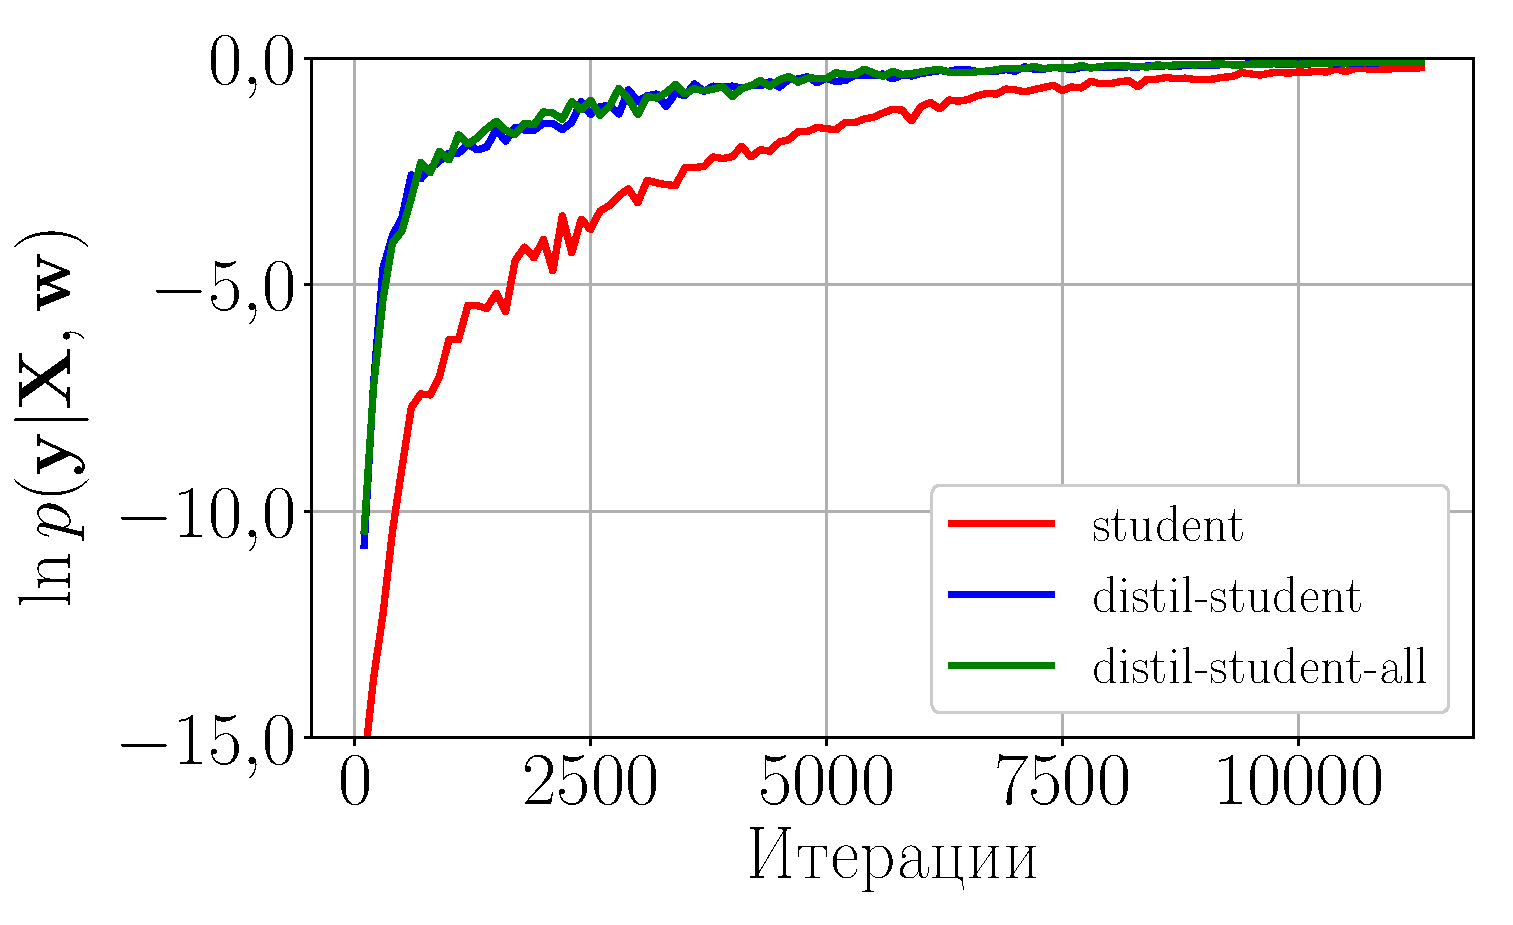
\includegraphics[width=0.4\textwidth]{figures/synthetic_likelihood_3_layers.eps}
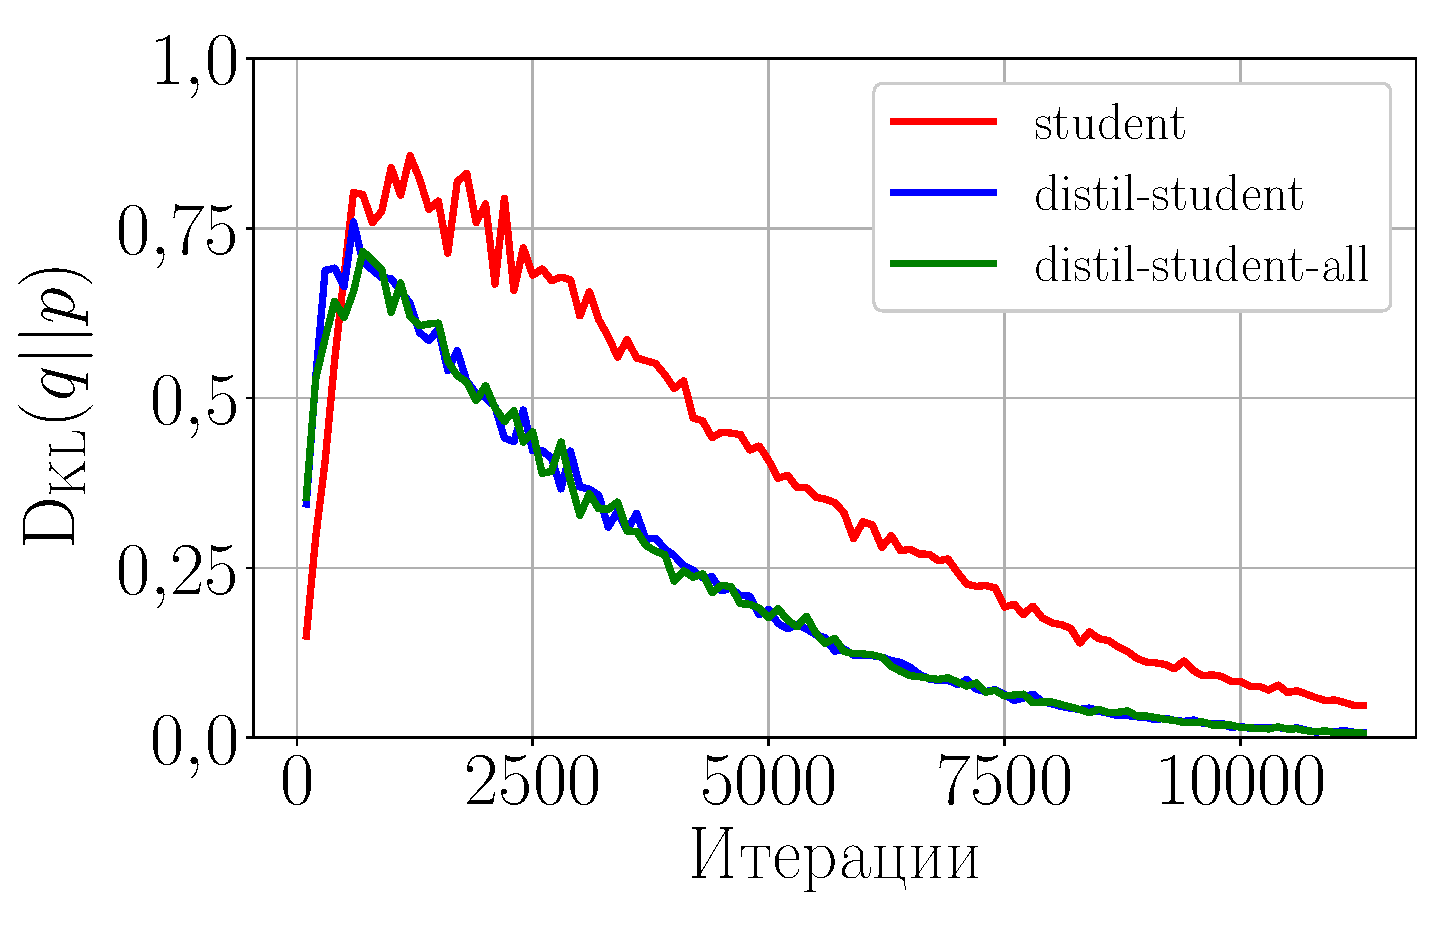
\includegraphics[width=0.4\textwidth]{figures/synthetic_D_KL_3_layers.eps}
\end{figure}
Первая конфигурация модели ученика. Дистиллированная модель имеет большее правдоподобие.

\begin{figure}[h!]
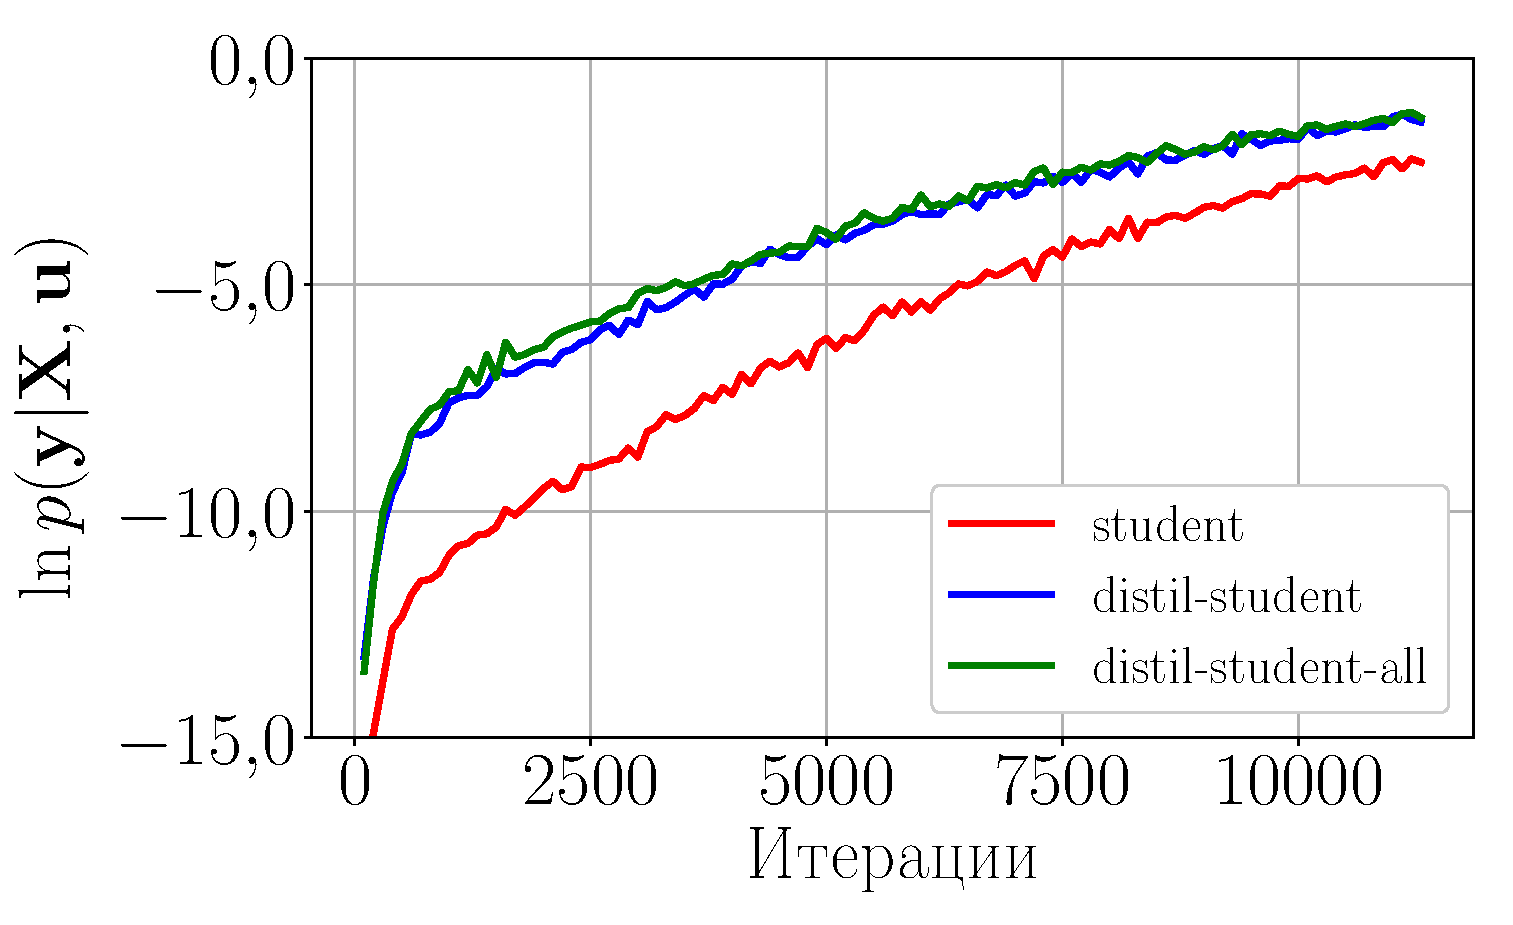
\includegraphics[width=0.4\textwidth]{figures/synthetic_likelihood_2_layers.eps}
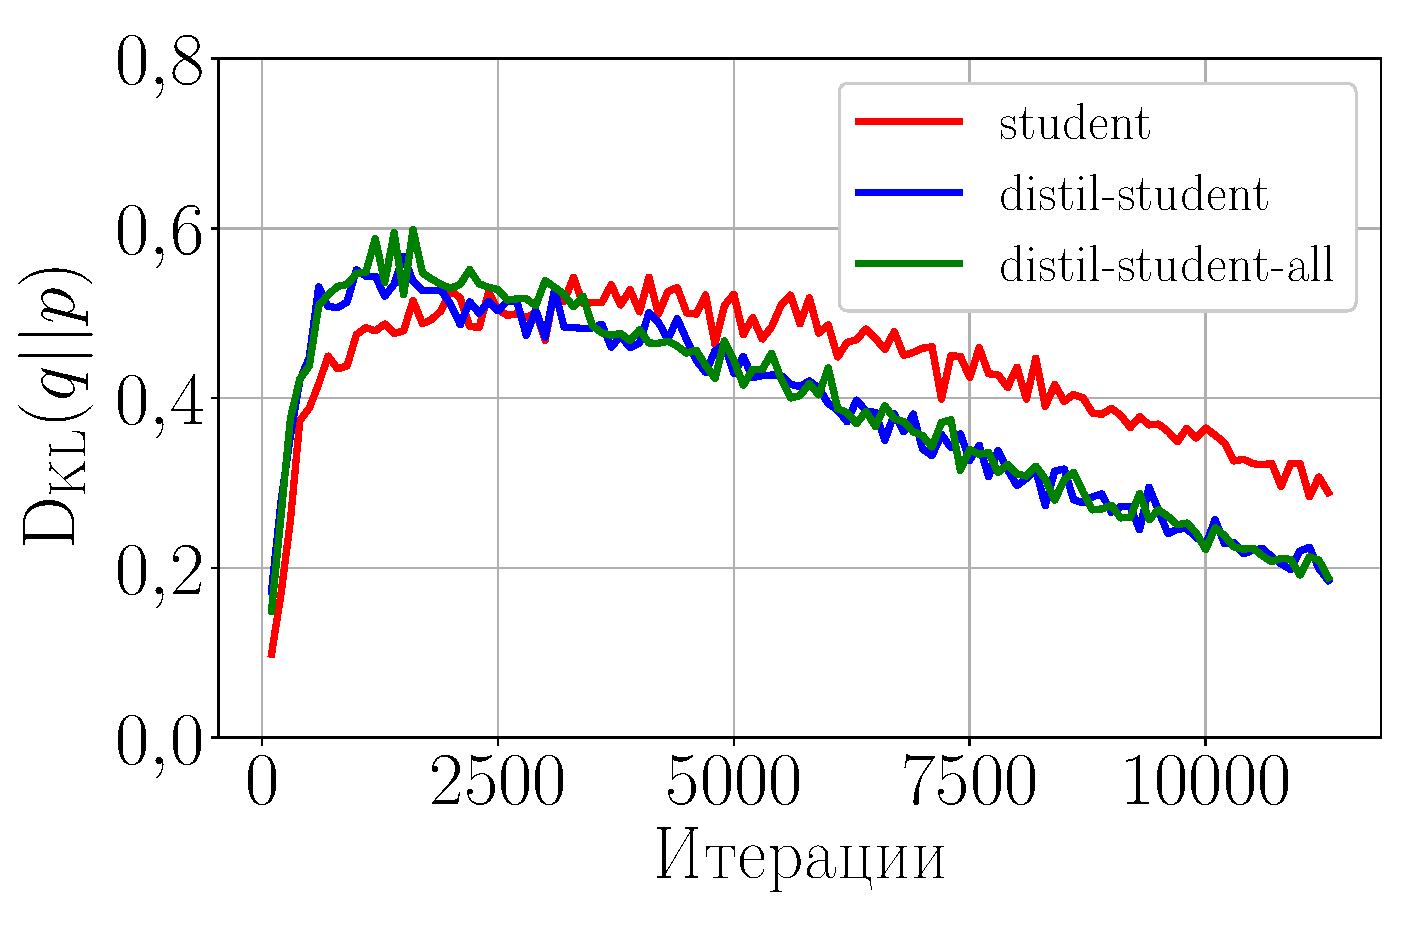
\includegraphics[width=0.4\textwidth]{figures/synthetic_D_KL_2_layers.eps}
\end{figure}
Вторая конфигурация модели ученика. Дистиллированная модель имеет большее правдоподобие.

\end{frame}
%----------------------------------------------------------------------------------------------------------

\begin{frame}{Сводная таблица вычислительного эксперимента: байесовская дистилляция}

\begin{table}[]
\begin{center}
\resizebox{\textwidth}{!}{
\begin{tabular}{|l|c|c|c|c|llll}

\cline{1-5}
                 & teacher           & student        & distil-student & distil-student-all &                           &                      &                      &                      \\ \cline{1-5}
\multicolumn{5}{|c|}{Эксперимент на синтетической выборке (удаление нейрона)}             &                      &                      &                      &                      \\ \cline{1-5}
Архитектура            & $[10,100,50,1]$   & $[10,10,10,1]$  & $[10,10,10,1]$ & $[10,10,10,1]$    &                      &                      &                      &                      \\ \cline{1-5}
Число параметров  & 6050                    & 210                   & 210                  & 210                      &                      &                      &                      &                      \\ \cline{1-5}
Разность площадей   &   -                         & 0                       & $\mathbf{16559}$              & $\mathbf{16864}$                  &                      &                      &                      &                      \\ \cline{1-5}
\multicolumn{5}{|c|}{Эксперимент на синтетической выборке (удаление слоя)}                    & \multicolumn{1}{c}{} & \multicolumn{1}{c}{} & \multicolumn{1}{c}{} & \multicolumn{1}{c}{} \\ \cline{1-5}
Архитектура            & $[10,100,50,1]$   & $[10,50,1]$       & $[10,50,1]$      & $[10,50,1]$          &                      &                      &                      &                      \\ \cline{1-5}
Число параметро    &   6050                       &       550                   &          550               &     550                        &                      &                      &                      &                      \\ \cline{1-5}
Разность площадей    &  -                          &  0                      &  $\mathbf{23310}$             & $\mathbf{25506}$                  &                      &                      &                      &                      \\ \cline{1-5}
\multicolumn{5}{|c|}{Эксперимент на выборке FashionMnist}                                                     &                      &                      &                      &                      \\ \cline{1-5}
Архитектура           & $[784,800,50,10]$& $[784,50,10]$   & $[784,50,10]$  & $[784,50,10]$      &                      &                      &                      &                      \\ \cline{1-5}
Число параметро    &   667700                     &     39700                     &      39700                   &      39700                       &                      &                      &                      &                      \\ \cline{1-5}
Разность площадей   & -                           & 0                       &  $\mathbf{1165}$               & $\mathbf{1145} $                   &                      &                      &                      &                      \\ \cline{1-5}
\end{tabular}
}
\end{center}
\end{table}

Для численного сравнения качества моделей выбрана разность площадей графика $\ln p\bigr(\textbf{y}|\textbf{X}, \textbf{w}\bigr)$. Чем больше значение тем лучше.

\end{frame}
%----------------------------------------------------------------------------------------------------------

\begin{frame}{Выносится на защиту}
\justifying
	\begin{enumerate}
	\justifying
	    \item Предложен байесовский метод обучения моделей ученика на основе моделей учителя.
        \item Предложен алгоритм построения модели на основе предобученных моделей.
        \item Предложен метод задания порядка на множестве параметров нейросетевых моделей на основе корреляции параметров.
        \item Предложен метод задания порядка на множестве параметров нейросетевых моделей при помощи оценки скорости сходимости параметров.
        \item Исследованы свойства дистилляции моделей глубокого обучения. Представлена вероятностная интерпретации дистиляции моделей глубокого обучения.
        \item Исследованы методы сопоставления параметрических моделей. Исследован метод получения априорного распределения параметров нейросети используя апостериорное распределение параметров исходной модели:
        \begin{itemize}
            \item различие в размерности слоев;
            \item различие в числе слоев.
        \end{itemize}
        
	\end{enumerate}

\end{frame}
%----------------------------------------------------------------------------------------------------------

\begin{frame}{Список работ автора по теме диссертации}
\justifying
{
\scriptsize
\textbf{Публикации ВАК по теме}

\begin{enumerate}
\item \textit{Грабовой А.В., Бахтеев О.Ю., Стрижов В.В.} Определение релевантности параметров нейросети // Информатика и ее применения, 2019.
\item \textit{Грабовой А.В., Бахтеев О. Ю., Стрижов В.В.} Введение отношения порядка на множестве параметров аппроксимирующих моделей // Информатика и ее применения, 2020.
\item \textit{A. Grabovoy, V. Strijov.} Quasi-periodic time series clustering for human // Lobachevskii Journal of Mathematics, 2020.
\item \textit{Грабовой А.В., Стрижов В.В.} Анализ выбора априорного распределения для смеси экспертов // Журнал Вычислительной математики и математической физики, 2021.
\item \textit{Грабовой А.В., Стрижов В.В.} Байесовская дистилляция моделей глубокого обучения // Автоматика и Телемеханика, 2021.
\item \textit{Грабовой А.В., Стрижов В.В.} Анализ моделей привилегированного обучения и дистилляции // (на рецензировании).
\item \textit{A. Grabovoy, T. Gadaev, A. Motrenko, V. Strijov} Numerical methods of minimum sufficient sample size estimation for linear models // (на рецензировании).
\item \textit{Bazarova A.I., Grabovoy A.V., Strijov V.V.} Analysis of the properties of probabilistic models in learning problems with an expert // (на рецензировании).
\end{enumerate}

\textbf{Выступление с докладом}
\begin{enumerate}
\item Автоматическое определение релевантности параметров нейросети // ИОИ-2018, 2018.
\item Поиск оптимальной модели при помощи алгоритмов прореживания // 61-я Всероссийская научная конференция МФТИ, 2018.
\item Анализ априорных распределений в задаче смеси экспертов // 62-я Всероссийская научная конференция МФТИ, 2019.
\item Введение отношения порядка на множестве параметров нейронной сети // ММРО-2019, 2019.
\item Привилегированная информация и дистилляция моделей // 63-я Всероссийская научная конференция МФТИ, 2020.
\item Задача обучения с экспертом для построение интерпретируемых моделей машинного обучения // ИОИ-2020, 2021.
\end{enumerate}
}
\end{frame}
%----------------------------------------------------------------------------------------------------------

\end{document} 